\section{Visibility of a sub satellite point} 

 
\textbf{Let’s consider the point P on Earth located at \textit{P} (0° latitude, 0°, longitude). }
\begin{itemize}
    \item[-] \textbf{Describe (in plain language) the conditions for the point P to be visible from the CubeSat.}

    In general, many aspects need to be taken into consideration when determining a point's visibility from a satellite. 
    Most importantly is \textit{Line of Sight}. 
    The CubeSat must have a clear and unobstructed line of sight to the point \textit{P}, which means that no part of Earth's surface should be blocking the view.

    The \textit{Orbital Path and Period} also play a vital role in the visibility of point \textit{P}. 
    The orbital path must be such that it brings the satellite into line of sight with the point \textit{P}. 
    E.g. very high inclination orbits, such as polar orbits, or geostationary orbits could be obtained in such a way that the point \textit{P} would never be visible.
    Since the CubeSat has a circular orbit and an inclination of 51,6 degrees, it will travel between the 51.6 degrees North and 51.6 degrees South, crossing the equator in between. 
    This means that at some points during it's orbits, the satellite will cross over the point \textit{P}.

    Realistically, \textit{Night and Day visibility} would also play arole. 
    While technically the point would be visible as long as the Line of Sight requirement is met, it is also important to remember in real-life applications that the point \textit{P} might not be visible to the CubeSat during night-time when it is dark.
    Depending on the instruments onboard the CubeSat and what is meant by "visible", i.e. visible to a communications array or visible in the sense that the satellite can take a clear image of the point \textit{P}.
    With the given orbital parameters, and an assumed orbital speed similar to the ISS (7.66 km/s), the CubeSat's orbital perioud would be about 92 min, meaning that it completes a whole orbit around Earth every 92 minutes. 
    As such, it would pass over the equator often enough that it would intersect with daytime.
    
    Simply put, the point \textit{P} is visible

    \autoref{fig:null} shows the real world location of the point \textit{P}.
    
    \begin{figure}[H]
        \centering
        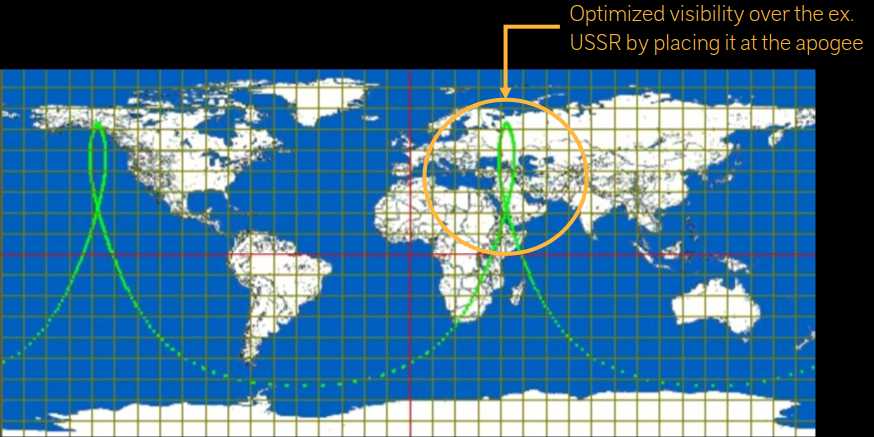
\includegraphics[width=0.75\linewidth]{Doc//Graphics/Molniya.png}
        \caption{Groundtrack of a Molniya orbit. The equator and prime meridian intersect at Null island (in red).}
        \label{fig:null}
    \end{figure}




    \item[-] \textbf{Describe an algorithm that allows to determine if the point P is visible from the CubeSat. } 

    The visibility can be determined based on the CubeSat and point \textit{P}'s position vectors in ECI and the orbital radius. 
    First the point \textit{P} needs to be expressed in ECI


    
    \item[-] \textbf{Code this algorithm and show, on a ground map, the points of the orbit which are visible from this point P.}
    \item[-] \textbf{What is the duration of the visibility for a satellite passing at the zenith of P?}
\end{itemize}

 
\vspace{0.5cm}
\begin{itemize}
    \item[-] \textbf{Express the vector (CubeSat, P) in satellite local orbital frame.}
    \item[-] \textbf{Describe an algorithm to compute the direction of the point P in local orbital reference frame.}
    \item[-] Code this algorithm and show, on a 3D plot, the vector wrt time over one orbit.
\end{itemize}